\documentclass[12pt,a4paper]{article}
\usepackage[utf8]{inputenc} %polskie znaki
\usepackage[T1]{fontenc}	%polskie znaki
\usepackage{amsmath}		%matematyczne znaczki :3
\usepackage{enumerate}		%Dodatkowe opcje do funkcji enumerate
\usepackage{geometry} 		%Ustawianie marginesow
\usepackage{graphicx}		%Grafika
\usepackage{wrapfig}		%Grafika obok textu
\usepackage{float}			%Allows H in fugire
\usepackage{hyperref}		%Allows hyperlinks
%\pagestyle{empty} 			%usuwa nr strony
\usepackage{todonotes}		%Todo notatki
\usepackage{lipsum}         %Lorem text
\usepackage{ntheorem}   	% for theorem-like environments
\usepackage{mdframed}   	% for framing
\usepackage{subcaption}		% subfigure (image placing)
\usepackage{pdfcomment}		% Komentarze (z bazowego pdf'a)
\usepackage{xparse}			% New commands with optional arguments
\usepackage{ifthen}			% If then - funkcje!
\usepackage{expl3}			% Deklarowanie zmiennych
\usepackage{pgf}			% Aktualne rachunki \pgfmathparse{}

\newgeometry{tmargin=2cm, bmargin=2cm, lmargin=2cm, rmargin=2cm} 

%Counter commands{
	\newcounter{counter} % Creates a new counter
	\setcounter{counter}{1} % Sets the counter to 5
	\newcommand{\counter}[1]{
		\arabic{#1} \stepcounter{#1} 
	}
	\newcommand{\counterreset}[1]{\setcounter{#1}{1}}
	%}
\newcounter{sub}
\setcounter{sub}{1}

%Define styles{
	\theoremstyle{break}
	\theoreminframepreskip{0.5cm}
	\theoremheaderfont{\bfseries}
	\newmdtheoremenv[%
	linecolor=white,%
	innertopmargin=\topskip,
	shadowsize=0,%
	innertopmargin=5,%
	innerbottommargin=5,%
	leftmargin=10,%
	rightmargin=10,%
	backgroundcolor=gray!20,%
	innertopmargin=0pt,%
	ntheorem]{zad}{Zadanie}
	
	\mdfdefinestyle{zadanie}{
		linecolor=white,%
		innertopmargin=5,%
		innerbottommargin=5,%
		leftmargin=10,%
		rightmargin=10,%
		backgroundcolor=gray!20,%
		innertopmargin=8,
		innerbottommargin=8,
		skipabove = 5,
	}
	\mdfdefinestyle{wzor}{
		linecolor=cyan,%
		linewidth=2pt,%
		innertopmargin=8,
		innerbottommargin=8,
		leftmargin=10,%
		rightmargin=10,%
		backgroundcolor = white, 
		fontcolor = black,
		skipabove = 5,
		skipbelow = 5,
	}
	%}

%Zadania templatex%{
	\newcommand{\Wzor}[1]{
		\begin{mdframed}[style=wzor]
			\centering #1
		\end{mdframed}
	}
	\newcommand{\ZadanieTextowe}[1]{
		\begin{mdframed}[style=zadanie]
			\textbf{Zadanie \counter{counter} } \\
			#1
		\end{mdframed}
	}
	\newcommand{\Zadanie}[2]{
		\begin{mdframed}[style=zadanie]
			\textbf{Zadanie \counter{counter} (0-#1) } \\
		\end{mdframed}
		#2
	}
	\newcommand{\SubZadanie}[2]{
		\begin{mdframed}[style=zadanie]
			\textbf{Zadanie \arabic{counter}.\counter{sub} (0-#1) } \\
		\end{mdframed}
		#2
	}
	\newcommand{\ZadanieABCD}[5]{
		\begin{mdframed}[style=zadanie]
			\textbf{Zadanie \counter{counter} (0-1)}
		\end{mdframed}
		\textbf{Dokończ zdanie. Zaznacz właściwą odpowiedź spośród podanych.}\\\\
		#1 \\\\
		\begin{tabular}{p{7cm} p{7cm}}
			\textbf{A. }#2&
			\textbf{B. }#3\\\\
			\textbf{C. }#4&
			\textbf{D. }#5\\
		\end{tabular}
	}
	\newcommand{\ZadanieABCDEF}[7]{
		\begin{mdframed}[style=zadanie]
			\textbf{Zadanie \counter{counter} (0-2)}
		\end{mdframed}
		\textbf{Uzupełnij zdanie. Wybierz \underline{dwie} właściwe odpowiedzi spośród oznaczonych literami A–F i wpisz te litery w wykropkowanych miejscach.} \\\\
		#1\\\\
		\begin{tabular}{p{7cm} p{7cm}}
			\textbf{A. }#2&
			\textbf{B. }#3\\\\
			\textbf{C. }#4&
			\textbf{D. }#5\\\\
			\textbf{E. }#6&
			\textbf{F. }#7\\\\
		\end{tabular}
	}
	
	\newcommand{\ZadaniePF}[3]{
		\begin{mdframed}[style=zadanie]
			\textbf{Zadanie \counter{counter} (0-2)}
		\end{mdframed}
		#1 \\\\
		\textbf{Oceń prawdziwość poniższych stwierdzeń. Wybierz P, jeśli stwierdzenie jest prawdziwe, albo F – jeśli jest fałszywe.} \\\\
		\PF{#2}{#3}
	}
	\newcommand{\PF}[2]{\setlength\arrayrulewidth{2pt}{
			\def\arraystretch{2}
			\begin{tabular}{|p{14cm}| c|c|}\hline
				#1 & {\Large P} & {\Large F}\\\hline
				#2 & {\Large P} & {\Large F}\\\hline
		\end{tabular}}
		\setlength\arrayrulewidth{0.5pt}
	}
	\newcommand{\PFEmpty}[2]{\setlength\arrayrulewidth{2pt}{
			\def\arraystretch{2}
			\begin{tabular}{|p{14cm}| c|}\hline
				#1 & {\Large $\dots$}\\\hline
				#2 & {\Large $\dots$}\\\hline
		\end{tabular}}
	}
	\newcommand{\Zadanietwoxtwo}[5]{
		\ZadanieTextowe{#1}
		\begin{tabular}{p{7cm} p{7cm}}
			\textbf{a)} #2&
			\textbf{b)} #3\\\\
			\textbf{c)} #4&
			\textbf{d)} #5\\\\
		\end{tabular}
	}
	\newcommand{\Zadanietwoxthree}[7]{
		\ZadanieTextowe{#1}
		\begin{tabular}{p{7cm} p{7cm}}
			\textbf{a)} #2&
			\textbf{b)} #3\\\\
			\textbf{c)} #4&
			\textbf{d)} #5\\\\
			\textbf{e)} #6&
			\textbf{f)} #7\\\\
		\end{tabular}
	}
	\newcommand{\Zadanietwoxfour}[9]{
		\ZadanieTextowe{#1}
		\begin{tabular}{p{7cm} p{7cm}}
			\textbf{a)} #2&
			\textbf{b)} #3\\\\
			\textbf{c)} #4&
			\textbf{d)} #5\\\\
			\textbf{e)} #6&
			\textbf{f)} #7\\\\
			\textbf{g)} #8&
			\textbf{h)} #9\\\\
		\end{tabular}
	}
	\newcommand{\Informacja}[1]{
		\counterreset{sub}
		\begin{mdframed}[style=zadanie]
			\textbf{Informacja do zadań \arabic{counter}.1 - \arabic{counter}.#1}
		\end{mdframed}
	}
	
	%}

\newcommand{\tg}{\text{tg}}
\newcommand{\ctg}{\text{ctg}}
\newcommand{\UkladRownan}[2]{
	$\left\{
	\begin{array}{l}
		#1 \\
		#2
	\end{array}
	\right.$
}

\begin{document}
{\Large Powtórzenie wybranych zagadnień:}
\begin{enumerate}[1)]
	\item {\large Wartość bezwzględna}
	
	Wyrażenie $$|x-a|<r$$ oznacza, że odległość $x$ od $a$ jest mniejsza od $r$. Np. mamy dla $$|x-7| < 15$$ 
	
	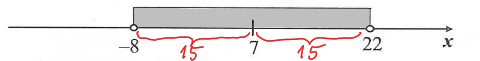
\includegraphics{r1.png}
	
	\item {\large Jak liczyć logarytmy?}
	
	Jednym ze sposobów jest liczenie z definicji:
	\Wzor{$\log_ab=c \qquad \Leftrightarrow \qquad a^c=b$}
	Np. chcemy policzyć $\log_2 16$
	\\\\
	Podstawiamy wyrażenie po lewej stronie: $$\log_2 16 = c,$$ czyli $$2^c=16$$
	$$c=4$$
	
	Drugim sposobem jest korzystanie ze wzorów (nie ma ich w tablicach maturalnych):
	
	\Wzor{$\log_aa^x=x \qquad \qquad \log_{a^y}a^x=\frac{x}{y}$}
	Dla powyższego przykładu otrzymujemy:
	$$\log_216=\log_22^4=4$$
	
	\item {\large Funkcje}
	
	X – zbiór \textbf{argumentów} \\
	Y – zbiór \textbf{wartości}
	\\\\
	Jeżeli podają nam argument, to chcemy odczytać wartość; jeżeli podają wartość, to chcemy odczytać argument.
	
	Np.\\ $f(x)<5$ – $f(x)=y$, zatem odczytujemy, kiedy funkcja jest mniejsza od 5 z osi \textbf{X} \\
	$f(2)=\dots$ – $f(2)=f(x)$, zatem $x=2$, odczytujemy wartość dla $x=2$
	\newpage
	\item {\large Funkcja liniowa}
	
	\Wzor{Warunek równoległości prostych\\
		$a_1=a_2$}
	\Wzor{Warunek prostopadłości prostych\\
		$a_1\cdot a_2=-1$}
	
	Interpretacja, jak rysować funkcję liniową:
	\\
	\begin{center}
		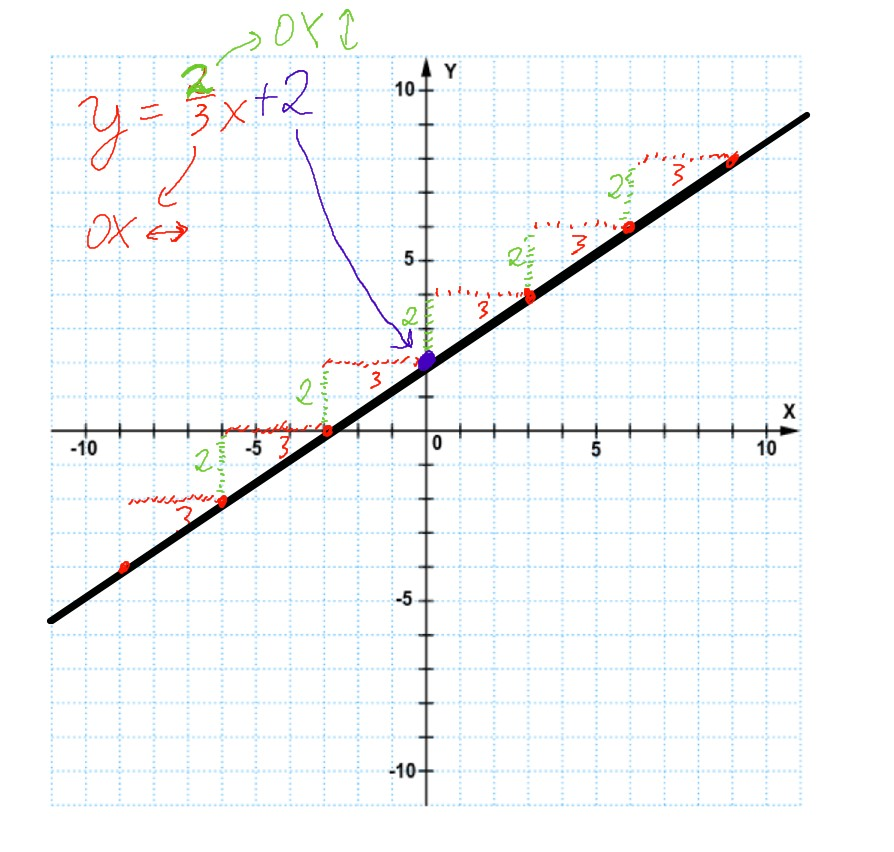
\includegraphics[scale=0.5]{r2.jpeg}
	\end{center}
	
	\item {\large Powtórka ze skali}
	
	Jak się zachowuje zwykła skala (długości) w stosunku do skali pól (P) i do skali objętości (V):
	
	$$(\text{dł})\:k = 2:3$$
	$$(\text{P})\:k^2 = 4:9$$
	$$(\text{V})\:k^3 = 8:27$$
	\newpage
	\item {\large Trygonometria}
	
	\begin{itemize}
		\item Funkcje trygonometryczne są zdefiniowane na trójkącie prostokątnym, ale można je wykorzystać także w trójkącie nieprostokątnym (np. tw. cosinusów)
		
		\item Jeżeli pojawi się tożsamość trygonometryczna z kwadratem, np. 
		$$\sin^3x + \sin x\cos^2x$$
		to NA PEWNO chodzi o ten wzór:
		\Wzor{Jedynka trygonometryczna\\ $\sin^2x+\cos^2x=1$}
		
		\item Jeżeli pojawi się $\tg x$ w tożsamości trygonometrycznej, to raczej chcemy go rozpisać ze wzoru:
		\Wzor{$\tg x = \frac{\sin x}{\cos x}$}
	\end{itemize}
	
	\item {\large Wielomiany}
	\begin{itemize}
		\item Metoda grupowania
		\item Metoda podstawiania ($t=x^2$, $t=x^3$)
		\item Twierdzenie Bezouta – przypomnienie
		
		Załóżmy, że mamy wielomian:
		$$W(x) = x^3 + 2x^2 - 12x + 8$$
		
		Twierdzenie to mówi, że jeżeli pod wielomian $W(x)$ za $x$ podstawimy coś (np. $x=1$), to przy dzieleniu wielomianu przez dwumian $(x-1)$ (1 jest miejscem zerowym dwumianu), reszta będzie równa $W(1)=1+2-12+8=-1=R$. Ponadto, jeżeli $W(a)=0$, to $a$ jest pierwiastkiem wielomianu i da się go rozłożyć na postać iloczynową. Np. $W(2)=8+8-24+8=0$, więc stosujemy schemat Hornera.
		
		\item Schemat Hornera
		
		\begin{center}
			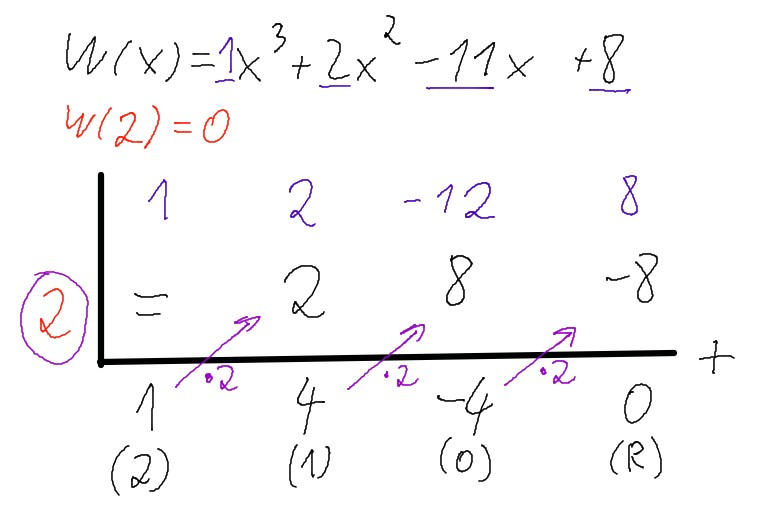
\includegraphics[scale=0.5]{r3.jpeg}
		\end{center}
		Możemy rozłożyć nasz wielomian do postaci:
		$$W(x)=(x-2)(x^2+4x-4)$$
		
	\end{itemize}
	
	\item {\large Ułamki algebraiczne}
	
	Pamiętaj o dziedzinie funkcji! Dzielenie przez 0 jest niedozwolone!
	
	\item {\large Ciągi}
	\begin{itemize}
		\item Warto pamiętać, że ciąg arytmetyczny da się rozpisywać w następujący sposób:
		$$a_{24} = a_1 + 23r$$
		
		\item Jeżeli dany jest trzywyrazowy ciąg arytmetyczny $(a_1,a_2,a_3)$, to warto skorzystać ze wzoru:
		\Wzor{$a_2=\frac{a_1+a_3}{2}$}
	\end{itemize}
\end{enumerate}
\vspace{2cm}
{\Large Ogólne porady:}
\begin{itemize}
	\item Jeżeli masz w zadaniu jakiś punkt (np. $A=(3,2)$), to możesz się spodziewać, że trzeba go podstawić do wzoru jakiejś funkcji (np. liniowej $y=ax+b$).
	\item Nie bój się korzystać z odpowiedzi podanych w zadaniu (typu ABCD), np. $x=3$ albo $m=-1$ – może coś z tego wyjdzie.
	\item Jeżeli możesz zrobić do zadania rysunek, zrób go dokładnie (od linijki). Może się okazać, że rozwiązanie wyjdzie z rysunku.
	\item Jeżeli masz zadanie z kombinatoryki i w odpowiedziach jest najwyższa liczba 30 ($+/-$), to zastanów się, czy nie warto wszystkich rozwiązań zapisać!
	\item Jeżeli nie masz pomysłu na zadanie (zwłaszcza te za 2–3 punkty), zastanów się, czy nie ma jakiegoś wzoru wykorzystującego dane z zadania (np. na pole, objętość, okrąg itp.)
\end{itemize}

	
\end{document}
